\documentclass[tikz]{standalone}

\usepackage[british]{babel}
\usepackage[utf8]{inputenc}
\usepackage{graphicx}
\usepackage{amsmath}
\usepackage{amssymb}
\usepackage{amsfonts}
\usepackage{bm}
\usepackage{color}
\usepackage[unicode]{hyperref}
\usepackage{multirow}
\usepackage{multicol}
\usepackage{tikz}
\usepackage{hyperref} % this is for url links
\usepackage{textcomp}
\usepackage{pgfplots}
\usetikzlibrary{calc,external,arrows}

%\usetikzlibrary{arrows,shapes}

\usepgfplotslibrary{polar}


\begin{document}

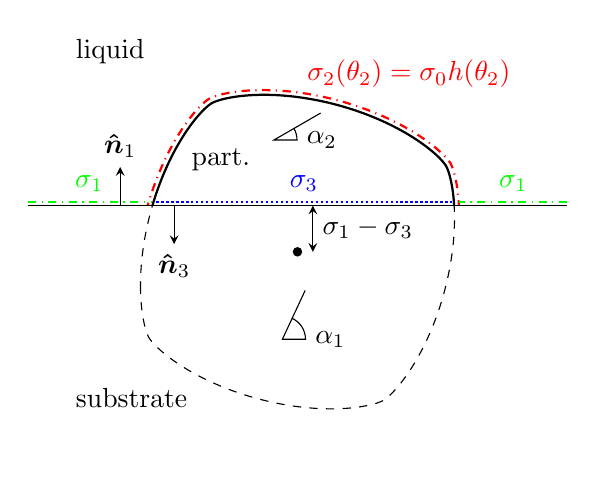
\begin{tikzpicture}[scale=1,font=\normalsize]
		\def\figxwidth{3.5}
		\begin{axis}[
			axis equal,
			disabledatascaling,
			axis line style={draw=none},
			xtick=\empty,
			ytick=\empty,
			xmin=-\figxwidth,xmax=\figxwidth,
			declare function={
				% yshift1=0;
				yshift1=-0.6;
				n=4;
				nsoa=0.9;
				rot1 = 30;
				RW = 0.7*3;
				d=nsoa/(n^2-1);
				aniso1(\t)=1+d*cos(n*(\t-rot1));
				daniso1(\t)=-n*d*sin(n*(\t-rot1));
				Wulffx1(\t) = RW*( aniso1(\t)*cos(\t) - daniso1(\t)*sin(\t) );
				Wulffy1(\t) = RW*( aniso1(\t)*sin(\t) + daniso1(\t)*cos(\t) );
			},
			]
			\begin{scope}
				\clip (axis cs: -\figxwidth,5) rectangle (axis cs:\figxwidth,0);
				\addplot[domain=-pi:pi, samples=150, smooth, thick] ({Wulffx1(deg(x))},{Wulffy1(deg(x))+yshift1});
				\addplot[domain=-pi:pi, samples=150, smooth, red, dash dot, thick] ({1.03*Wulffx1(deg(x))},{1.03*Wulffy1(deg(x))+yshift1});
			\end{scope}
			
			\begin{scope}
				\clip (axis cs: -\figxwidth,-5) rectangle (axis cs:\figxwidth,0);
				\addplot[domain=-pi:pi, samples=150, smooth,dashed] ({Wulffx1(deg(x))},{Wulffy1(deg(x))+yshift1});
			\end{scope}
			
			\path coordinate (C1) at (axis cs:0,yshift1);
			\path coordinate (B1) at (axis cs:-\figxwidth,0);
			\path coordinate (B2) at (axis cs:\figxwidth,0);
			\path coordinate (zz) at  (axis cs:0,0);
			
			% interface specifications
			\draw (B1) -- (B2);
			\draw[green, dash dot, thick] (axis cs:-\figxwidth,0.05) -- node[midway, above] {$\sigma_{1}$} (axis cs:-1.9,0.05);
			\draw[red] (axis cs:0,1.4) node[above right] {$\sigma_{2}(\theta_{2})=\sigma_0 h(\theta_2)$} ;
			\draw[green, dash dot, thick] (axis cs:\figxwidth,0.05) -- node[midway, above] {$\sigma_{1}$} (axis cs:2.1,0.05);
			\draw[blue, densely dotted, thick] (axis cs:-1.83,0.05) -- node [midway, above] {$\sigma_{3}$} (axis cs:2.0,0.05);
			
			\draw[-stealth] (axis cs:-2.3,0) -- (axis cs:-2.3,0.5) node [above] {$\bm{\hat{n}}_1$};
			\draw[-stealth] (axis cs:-1.6,0) -- (axis cs:-1.6,-0.5) node [below] {$\bm{\hat{n}}_3$};
			
			
			\draw[stealth-stealth] (axis cs:0.2,0) -- (axis cs:0.2,yshift1/2) node [right] {$\sigma_1-\sigma_3$} -- (axis cs:0.2,yshift1);
			
			
			\draw[fill] (C1) circle (1.5pt);

			\draw (0.3,1.2) -- ++(-150:0.7) -- ++(0:0.3) node [right] {$\alpha_2$} arc (0:30:0.3) ;
			\draw (0.1,-1.1) -- ++(65-180:0.7) -- ++(0:0.3) node [right] {$\alpha_1$} arc (0:65:0.3) ;
			
			\draw (-3,2) node [right] {liquid};
			\draw (-3,-2.5) node [right] {substrate};
			\draw (-1.5,0.6) node [right] {part.};
		\end{axis}
	\end{tikzpicture}

    
\end{document}
